\documentclass{atistandalonetask}
\usepackage{atistandard}

\begin{document}
  \begin{atiTask}[
    title = Periodische Fortsetzung
  ]


	\begin{atiSubtasks}
		\item Skizzieren Sie die Funktion $f(t)=4-t^2$ im Bereich $-2\leq t\leq 2$ und skizzieren Sie eine periodische Fortsetzung.
		\item Berechnen Sie die Fourierreihe zu $f(t)$.
		\item Verifizieren Sie das \textsc{Parseval}sche Theorem für dieses Beispiel.
	\end{atiSubtasks} 
	\atiNote{\[\sum _{n=1}^\infty\frac{1}{n^4}=\frac{\pi^4}{90}\]}
  \end{atiTask}
  \begin{atiSolution}
  Lösung folgt
   %   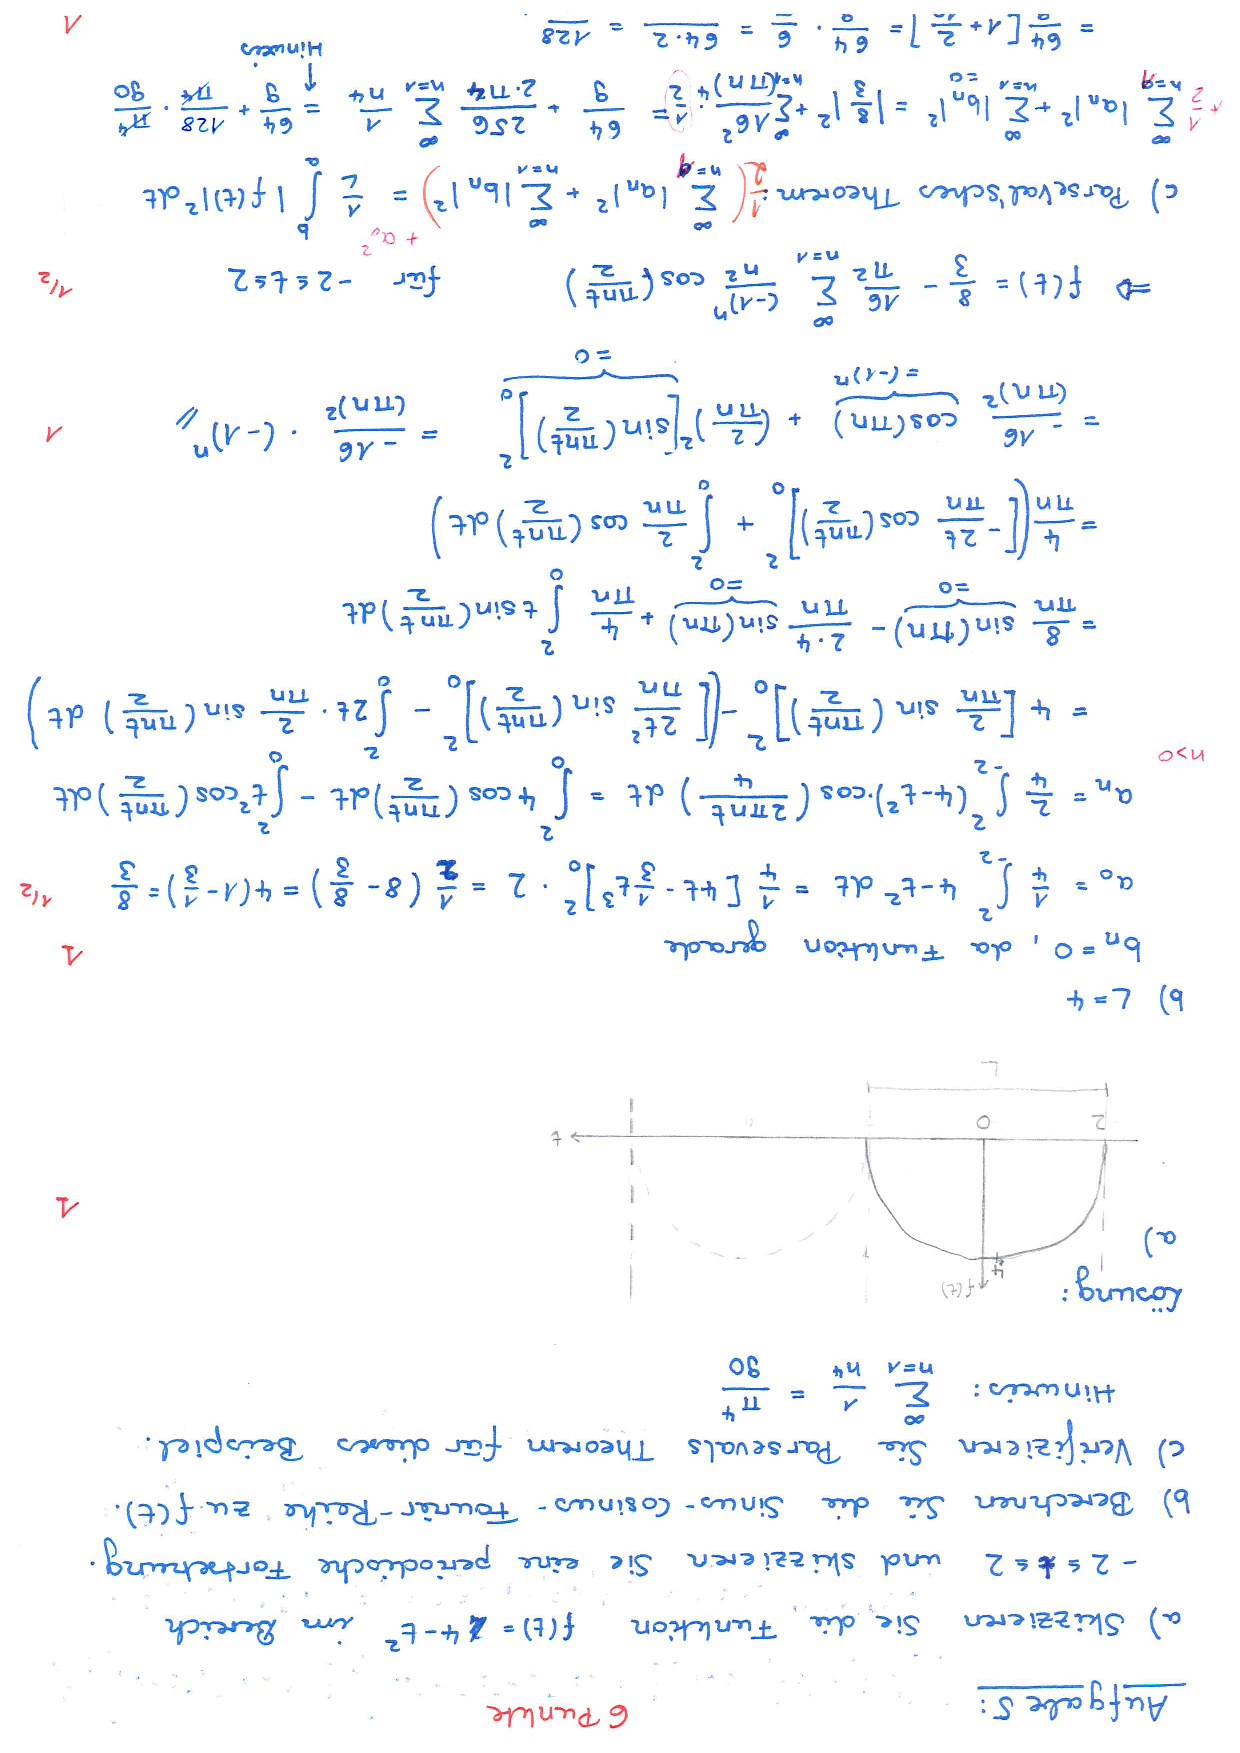
\includepdf[pages=-]{solution-fourier_vi.pdf}
  \end{atiSolution}
\end{document}